% !TeX encoding = UTF-8

\chapter{核心定理推导补充}

本附录演示规范 1.11 节要求的附录格式：附录编号与附录标题各占一行并居中排列；附录中的公式、图和表分别自动编号为 \texttt{(A1)}、\texttt{图 A1}、\texttt{表 A1}。

在满足 $L$-光滑性假设条件下，局部更新误差的一步递推不等式可写为：
\begin{equation}
  \mathbb{E}\!\left[\|\mathbf{w}_k^{t, r} - \mathbf{w}^t\|^2\right]
  \le 5 E \eta_t^2 \left(\sigma_g^2 + 6 E \zeta^2\right),
  \label{eq:appendix-lemma}
\end{equation}
式~(\ref{eq:appendix-lemma}) 的编号自动采用 \texttt{(A1)} 形式。

\begin{table}[htbp]
  \centering
  \caption{附录补充实验数据集统计特征}
  \label{tab:appendix-dataset}
  \begin{tabular}{@{}l c c c@{}}
    \toprule
    数据集 & 类别数 & 训练样本量 / 条 & 测试样本量 / 条 \\
    \midrule
    Fashion-MNIST & 10 & 60\,000 & 10\,000 \\
    CIFAR-10      & 10 & 50\,000 & 10\,000 \\
    \bottomrule
  \end{tabular}
\end{table}

\begin{figure}[htbp]
  \centering
  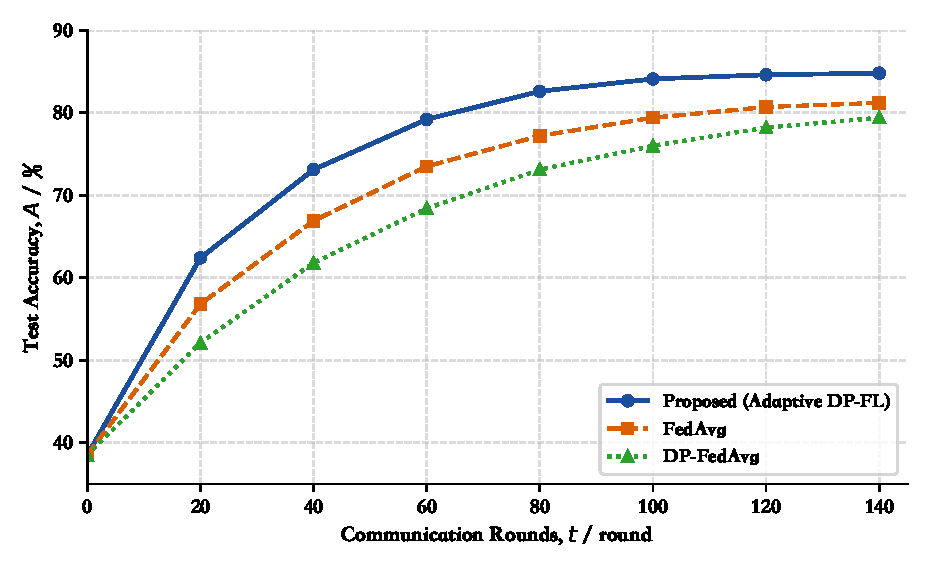
\includegraphics[width=0.68\textwidth]{figures/demo-curve.pdf}
  \caption{附录补充收敛稳定性验证曲线}
  \label{fig:appendix-fig}
\end{figure}
